\def\sectionautorefname{Section}
\def\subsectionautorefname{Subsection}

% Attempt to create appendix table of contents
\doparttoc % Tell to minitoc to generate a toc for the parts
\faketableofcontents % Run a fake tableofcontents command for the partocs

\section{Introduction}

% A few sentences placing the work in high-level context. Limit it to a few paragraphs at most; your report is on reproducing a piece of work, you don’t have to motivate that work.

Recently, \acp{GNN} became a pivotal topic in AI research \citep{Keramatfar2022}. While the domain itself develops rapidly, the notion of fairness in the context of graph learning lags behind \citep{Khajehnejad2022}. When graph-based systems neglecting fairness are deployed in the real world, protected groups may become unjustly mistreated. 

% In order to model complex relationships appearing in the world around us, one can seldom limit themselves to the use of simple data structures, such as vectors and matrices. Therefore, the introduction of graph methods proved indispensable for numerous tasks, including disease spread prediction, logistic route optimization, and molecular fingerprint learning \citep{Zhou2018}. Recently, \acp{GNN} became a pivotal topic in AI research \citep{Keramatfar2022}. While the domain itself develops rapidly, the notion of fairness in the context of graph learning lags behind \citep{Khajehnejad2022}.

% When graph-based systems neglecting fairness are deployed in the real world, protected groups may become unjustly mistreated. The disregard for fairness manifests differently depending on the task. For example, when choosing a limited number of nodes in a social network to maximize information spread, an optimal solution in terms of accuracy can lead to the information never reaching members of smaller, more secluded groups. This may result in an unequal access to opportunities, such as loan offers and job advertisements, which may further deepen disparities in the long run. 

FairWalk \citep{Rahman2019} falls among the earliest attempts at mitigating such issues. In particular, it provides probabilities for which edge to select when generating random walks through the graph, an essential part of many current graph learning methods. \citet{Khajehnejad2022} followed up on its ideas by designing CrossWalk, a more complex strategy which considers the context of nodes when weighting edges leading towards them.

In this paper, we verify the authors' claims by re-implementing CrossWalk and reproducing their results. We provide three main contributions:
\begin{enumerate}
    \item \textbf{Full re-implementation.} We re-implement the full pipeline from scratch. The motivation is twofold: (1) arrival to the same conclusions using two independent implementations strengthens the claims; (2) it makes building on top of the original work more easy and viable. In support of the last point, we develop an MIT-licensed package allowing the application of CrossWalk to \ac{DGL} graphs with a single line of code.
    % \item \textbf{Full re-implementation.} We re-implement the full pipeline from scratch using industry-standard frameworks, namely PyTorch and DGL (see \autoref{subsec:exp_code}). The motivation for full re-implementation is twofold: (1) arrival to the same conclusions using two independent implementations strengthens the claims; (2) it makes building on top of the original work more easy and viable. In support of the last point, we develop an MIT-licensed package allowing the application of CrossWalk to DGL graphs with a single line of code.
    \item \textbf{Robustness check.} In the original paper, every experiment is run 5 times and no variation measure is provided. We statistically validate the original results by running the experiments over 50 independent runs and reporting on their variability.
    \item \textbf{Theoretical extension.} While implementing the package, we found problematic edge cases that were not treated in the original CrossWalk algorithm. Therefore, we dived into the theory and came up with an extended formulation with useful probabilistic properties.
\end{enumerate}

\section{Scope of reproducibility}
\label{sec:claims}

% Introduce the specific setting or problem addressed in this work, and list the main claims from the original paper. Think of this as writing out the main contributions of the original paper. Each claim should be relatively concise; some papers may not clearly list their claims, and one must formulate them in terms of the presented experiments. (For those familiar, these claims are roughly the scientific hypotheses evaluated in the original work.)

% A claim should be something that can be supported or rejected by your data. An example is, ``Finetuning pretrained BERT on dataset X will have higher accuracy than an LSTM trained with GloVe embeddings.'' This is concise, and is something that can be supported by experiments. An example of a claim that is too vague, which can't be supported by experiments, is ``Contextual embedding models have shown strong performance on a number of tasks. We will run experiments evaluating two types of contextual embedding models on datasets X, Y, and Z."

% Claims should be clearly separated and organized into a list.

The paper \textit{CrossWalk: Fairness-Enhanced Node Representation Learning} by \citet{Khajehnejad2022} contributed to the field by proposing CrossWalk, a general graph-processing method designed to enhance group fairness of algorithms based on stochastic traversal of a graph. In their paper, the authors study the application of CrossWalk to random walk based node embedding methods, namely DeepWalk \citep{Perozzi2014} and Node2Vec \citep{Grover2016}. CrossWalk is discussed in more detail in \autoref{sec:crosswalk}.
% Which claim?
%  Version 1
In their abstract, the authors summarize their main claims as follows: 

"\textit{Extensive experiments show the effectiveness of our algorithm to enhance fairness in various graph algorithms, including influence maximization, link prediction and node classification in synthetic and real networks, with only a very small decrease in performance.}" \cite{Khajehnejad2022}. \\

More details about these experiments can be found in \autoref{sec:methodology}. We separate these claims into two sub-claims, which we wish to verify:
\begin{itemize}
    \item \textbf{Claim 1: Fairness-enhancing property.} The authors claim that the application of CrossWalk in all the experiments referenced above leads to enhanced fairness as measured by disparity, compared to both FairWalk and no reweighting-strategy as baselines.
    \item \textbf{Claim 2: Performance-conserving property.} The authors claim that the application of CrossWalk in all the experiments referenced above only leads to very small decreases in performance. We interpret this as the performance of every experiment is reduced by at most 10\% when applying crosswalk, compared to both FairWalk and no reweighting-strategy as baselines.
\end{itemize}

% Subsequently, they evaluate CrossWalk in terms of accuracy and disparity, their fairness metric of choice, on three general graph-related tasks, specifically influence maximization, node classification, and link prediction.

% K: Removed / Merged the paragraph below into section 3
% \citet{Khajehnejad2022} designed CrossWalk to rectify situations where group fairness may be lacking. In principle, one can apply CrossWalk to any graph, directed or undirected, containing weighted edges between nodes. 
% When processing the graph, CrossWalk adjusts edge weights such that edges either leading from a given node closer to its group's borders or directly crossing such borders are amplified. In consequence, stochastic graph algorithms traversing the graph have higher chance of leaving the group of the initial node and visiting nodes belonging to other groups. 

% Our aim is to confirm the conclusions that \citet{Khajehnejad2022} arrived to in their paper. To be precise, we wish to verify the following:

% \begin{itemize}
%     \item \textbf{Influence maximization.} Compared to both simple and FairWalk-enhanced DeepWalk node embeddings, CrossWalk provides a significant improvement in disparity without affecting the total influence on 2-grouped synthetic, 3-grouped synthetic, Twitter, and Rice-Facebook datasets. Compared to simple Node2Vec node embeddings, FairWalk and CrossWalk provide similar improvement in disparity without affecting the total influence on Rice-Facebook dataset.
%     \item \textbf{Node classification.} Compared to both simple and FairWalk-enhanced DeepWalk node embeddings, CrossWalk provides a significant improvement in disparity without affecting the total accuracy on Rice-Facebook dataset.
%     \item \textbf{Link prediction.} Compared to both simple and FairWalk-enhanced DeepWalk node embeddings, CrossWalk provides a significant improvement in disparity without affecting the total accuracy on Twitter and Rice-Facebook datasets.
% \end{itemize}

\section{CrossWalk}
\label{sec:crosswalk}

% However, to make things more difficult: In principle, this can also happen when v is not a "Karen"-node, because estimating colorfulness is a stochastic process based on random walks. It is possible that even when v has neighbors z in N(v) that have neighbors u in N(z) of a different color, the colorfulness for all u is estimated as 0 if none of the random walks for estimating colorfulness used the edge w_zu connecting z to its differently-colored neighbor, and thus z's colorfulness is estimated as 0. 

% Sorry for posting so much. But here's an easier explanation to understand why this case of the sum in the denominator can be 0 can happen to any node v whose neighbors z in the denominator's sum have at least 1 node u with the same color, i.e. c(u)==c(z):

% For all of these z, when estimating colorfulness, all random walks could theoretically go back and forth between z and u, and thus z's colorfulness would be estimated as 0.

% by doing this, we ensure that isolated nodes do not have to be removed ~ an improvement of the original algorithm which would break - authors removed the isolated nodes upfront and they do (not?) mention this practice in the paper at all

\subsubsection*{Original motivation}

As their main contribution, \citet{Khajehnejad2022} introduced CrossWalk, an edge reweighting algorithm designed to enhance group fairness in tasks based on node embeddings generated by random walks through graphs.

\subsubsection*{The CrossWalk algorithm}


Random walks are part of techniques to obtain node embeddings like Node2Vec and Deepwalk. 
In this context, an edge weight $w_{uv}$ corresponds to the probability of choosing $v$ as the node following $u$ during random walks.
Given groups defined by some protected characteristic of choice, such as gender or race, the method amplifies edge weights leading towards nodes that are in different groups than the source node, and towards nodes in the proximity of different groups. 
Consequently, random walks traverse group boundaries more often.
% This ensures that algorithms traversing the graph in a stochastic manner are more likely to escape the boundaries of groups defined by the protected characteristic. 
% Given groups defined by some protected characteristic of choice, such as gender or race, the method amplifies the edges leading to and outside group boundaries while reducing the edges leading closer to group centers. 
The author's intention of applying CrossWalk in this setting is to obtain node embeddings that are more fair when evaluated in the context of a downstream task.
The effect the application of CrossWalk has on node embeddings is visualized in \autoref{fig:visualization-embeddings} in the appendix.
% TODO: Fix title of figure below or replace

\subsubsection*{Motivation for extension}
\label{sec:motivation}

When reproducing the paper, we encountered disparities between the CrossWalk reweighting formula found in \cite[Equation~4]{Khajehnejad2022}, the CrossWalk pseudo-algorithm found in \cite[Algorithm~1]{Khajehnejad2022}, and the CrossWalk implementation available on GitHub \citep{Khajehnejad2022-github}. 
In particular, the pseudo-code covers an additional case that is neglected in the formula. Moreover, the public implementation addresses an additional case which is not mentioned throughout the original paper. Further, implementing CrossWalk according to the original formula and pseudocode leaves room for edge cases in which a division by zero may occur.
% These disparities make it difficult to re-implement the method as the existence of such edge cases and their nature remain unclear from the code.

The main motivation for proposing adaptations to the CrossWalk algorithm lie in resolving these issues and ambiguities. We hope that this helps future researchers to decide whether CrossWalk is suited for their application.

\subsubsection*{Design goals for extension}
Our proposed algorithm is designed such that a) the algorithm handles edge cases gracefully and b) yields nice probabilistic properties, while c) making only minimal changes to the authors' original approach, prioritizing their algorithm as originally implemented in \citep{Khajehnejad2022-github} over their pseudocode and formulas. In practice, the two versions barely differ, as the extensions are mainly about handling of edge cases. The results of our experiments confirming the similarity are in \autoref{fig:ours-vs-theirs} in the Appendix.

With the introduction our changes, we increase the number of cases in which the graph obtained from CrossWalk is guaranteed to be \textit{probabilistic}, which makes it more feasible to be applied in more areas. This guarantee removes the necessity to normalize the weights before treating them as transition probabilities when doing e.g. random walks, enabling more efficient implementations of CrossWalk based applications.

Further, the probabilistic property of a graph may be useful in applications outside of random walks discussed here.  For example, future research may investigate reweighting transition probabilities in Markov chains with the CrossWalk strategy, in cases where the nodes (states) are assigned to different groups, and an increase of transitions between states of different groups is desired.


\subsubsection*{Extension scope}
In the following section, we present an extended formulation of the CrossWalk algorithm to address the issues described above. For this, we extend the equations and pseudo-code and make slight notational adjustmends. Finally, we show a valuable property of the reweighting strategy.
% In the following section, we present an extended theoretical framework addressing the above-mentioned issues. 
% Firstly, we extend both the reweighting formula and pseudo-code to be consistent for all possible cases. 
% Secondly, we make slight notational adjustments  for easier understanding and implementation of CrossWalk. 
% Finally, we propose and prove a theorem identifying an inherently valuable characteristic of the reweighting strategy. 

\subsubsection*{Extension proposal}
% % TODO: Use same formatting as Definition

In this section we assume weighted and directed graphs. However, the definitions and results can easily be extended to undirected graphs (by assuming each edge to have an anti-parallel counterpart), and unweighted graphs (by assuming all initial edge weights to be equal).

Let $G = (V, E, w)$ be a weighted graph, where $V$ is the graph's node set, $E$ is the set of edges between the nodes, and $w_{vu} > 0$ are positive edge weights for all edges $(v, u) \in E$. We define $\mathcal{N}(v)$ as the set of neighbors of node $v \in V$ for which an edge from $v$ to $u$ exists. We define $c(z)$ as a function returning the \textit{color} of node $z \in V$. In the context of fairness, color refers to the group defined by the protected characteristic that $z$ belongs to. Let $N_v^c \subseteq \mathcal{N}(v)$ be the set of neighbors of node $v$ of color $c$. Then, we can also define $R_v = \{ c(u) \ | \ u \in \mathcal{N}(v) \} \setminus c(v)$, as the set of colors appearing in the neighborhood of node $v$ that are different from the color of $v$.

\begin{definition}[colorfulness]\label{def:colorfulness}
We define \textit{colorfulness} of node $v$, a measure of proximity of $v$ to nodes belonging to other groups, as a function $m(v): V \to \langle 0, 1 \rangle$.  Colorfulness is estimated by taking $r$ random walks of length $d$ from node $v$ using the original edge weights $w$. It is calculated as 
\begin{equation}\label{eq:colorfulness}
m(v) = \frac{\sum_{j = 1}^r \sum_{u \in \mathcal{W}_v^j} \mathbb{I}[c(v) \neq c(u)]}{rd},
\end{equation}
where $\mathcal{W}_v^j$ is a set of nodes in the $j$-th random walk from $v$ and $\mathbb{I}$ is an indicator function.
\end{definition}

% \begin{remark}
% Intuitively, colorfulness calculates the fraction of nodes belonging to other groups which are located close to the node $v$ itself.
% \end{remark}

Below are our proposed equations for computing each edge's new weight with the CrossWalk algorithm. A pseudocode-based on these equations is provided in \autoref{alg:crosswalk} in the Appendix. Note that our extensions to the formulas proposed originally in \cite[Equation~4]{Khajehnejad2022} are marked in {\color{pinkcolor} pink color}, and are briefly commented on below.

% The reweighting strategy of CrossWalk is determined by each node's neighborhood. By blindly following the original formula in \cite[Equation~4]{Khajehnejad2022}, however, one quickly runs into an important issue. If colorfulness of at least one neighboring node in each group appearing in the neighborhood of a node is not larger that zero, the reweighting strategy performs division by zero. Authors partially account for this issue in their implementation, but they never mention it in the paper. To solve the issue, we propose to normalize the weights as

\begin{subnumcases}{n_{vu} =}
    \frac{w_{vu} m(u)^p}{\sum_{z \in N_v^{c(u)}} w_{vz} m(z)^p}, & {\color{pinkcolor} if $\exists z \in N_v^{c(u)} : m(z) > 0,$ \label{eq:crosswalk:norm1}} \\
    {\color{pinkcolor}\frac{w_{vu}}{\sum_{z \in N_v^{c(u)}} w_{vz}}} & {\color{pinkcolor} otherwise.} 
    \label{eq:crosswalk:norm2}
\end{subnumcases}

% where hyperparameter $p$ determines the degree to which edges leading closer to group boundaries are upweighted. If there exists at least one neighbor of node $v$ from a particular group with an estimated colorfulness of more than zero, the standard CrossWalk normalization procedure is employed (\autoref{eq:crosswalk:norm1}). However, once a group of neighbors does not have any representative for which the estimated colorfulness is larger then zero, colorfulness must be dropped from the normalization procedure for that particular group (\autoref{eq:crosswalk:norm2}).

% In the original formula found in \cite[Equation~4]{Khajehnejad2022}, the authors address only the situation where the node whose outgoing edges are reweighted \textbf{has at least one same-colored and one differently-colored neighbor (Equations~\ref{eq:crosswalk:base1}~and~\ref{eq:crosswalk:base2})}. Then, CrossWalk reweights the edges as 
\begin{subnumcases}{w'_{vu} =}
    (1-\alpha) n_{vu}, & if $c(v) = c(u) {\color{pinkcolor} \ \wedge \ \mathcal{N}(v) \neq N_v^{c(v)}},$ \label{eq:crosswalk:base1} \\
    \frac{\alpha}{|R_v|} n_{vu}, & if $c(v) \neq c(u) {\color{pinkcolor} \ \wedge \ \mathcal{N}(v) \neq \left( \bigcup_{c \in R_v} N_v^{c} \right)},$ \label{eq:crosswalk:base2} \\
    {\color{pinkcolor} n_{vu},} & {\color{pinkcolor} if $c(v) = c(u) \ \wedge \ \mathcal{N}(v) = N_v^{c(v)},$} \label{eq:crosswalk:add1} \\
    {\color{pinkcolor} \frac{1}{|R_v|} n_{vu},} & {\color{pinkcolor} if $c(v) \neq c(u) \ \wedge \ \mathcal{N}(v) = \left( \bigcup_{c \in R_v} N_v^{c} \right).$} \label{eq:crosswalk:add2} 
\end{subnumcases}
% where hyperparameter $\alpha$ determines how much the edges leading from the group of node $v$ to different groups are upweighted. In the original pseudo-algorithm found in \cite[Algorithm~1]{Khajehnejad2022}, the authors additionally account for the case where the node whose outgoing edges are reweighted \textbf{only has differently-colored neighbors (\autoref{eq:crosswalk:add2})}. However, they do not account for this in their formula or in the text. Finally, the case where the node \textbf{only has same-colored neighbors (\autoref{eq:crosswalk:add1})} is fully omitted from the paper and appears only in the original code without proper commentary. For these two cases, CrossWalk reweights edges as
% {\color{pinkcolor} 
% \begin{subnumcases}{w'_{vu} =}
%     n_{vu}, & if $c(v) = c(u) \ \wedge \ \mathcal{N}(v) = N_v^{c(v)},$ \label{eq:crosswalk:add1} \\
%     \frac{1}{|R_v|} n_{vu}, & if $c(v) \neq c(u) \ \wedge \ \mathcal{N}(v) = \left( \bigcup_{c \in R_v} N_v^{c} \right),$ \label{eq:crosswalk:add2} 
% \end{subnumcases}
% }
% We will probably not use the paragraph below as it is replaced by Kieron's below it
% An extended pseudo-code employing the changes can be found in \autoref{alg:crosswalk}. When CrossWalk is fully implemented such that it accounts for all of the aforementioned cases, the methodology recovers a valuable property common to graphs of Markov chains. In particular, independent of the original weights of the outgoing edges of a node, they will always sum up to one after being processed by CrossWalk. In consequence, they can be interpreted as probabilities of hopping from a particular node to its neighbors. The original paper does not delve deeper into this property. However, we believe that it creates a solid theoretical basis for application of CrossWalk to other stochastic graph-based algorithm as well. Therefore, we choose to formalize this property.

In the code provided with the original paper, the authors added $0.001$ when estimating a node's colorfulness with \autoref{eq:colorfulness}. 
This prevented the possibility of dividing by zero in \autoref{eq:crosswalk:norm1}, but was not mentioned in the formulas or pseudocode.
Instead of adding that term, we propose imposing a condition to \autoref{eq:crosswalk:norm1} and adding \autoref{eq:crosswalk:norm2} to handle these cases.

Further, we impose additional conditions to Equations \ref{eq:crosswalk:base1} and \ref{eq:crosswalk:base2} (marked in green) and propose Equations \ref{eq:crosswalk:add1} and \ref{eq:crosswalk:add2} to handle these additional cases, respectively. \autoref{eq:crosswalk:add1} is an entirely new proposal of ours to make \autoref{th:theorem1} hold, while \autoref{eq:crosswalk:add2} was already included in the authors' original implementation and pseudocode, but was missing in the mathematical notation.

% oh, and just for completeness, they also use the mean performance over all samples, and not the mean performance over all groups

% Authors originally removed isolated edges, however, our extension allows for them -> however, it is necessary to mention that one must account for their occurrence by either adding self-connections or requiring random walks to repeat the same node if there is no other node to move to

% Can you make sure to word this case such that edges with outgoing weights=0 are caught as well? No outgoing edges and no outgoing edges with weight !=0 might sound very similar, but might be a worthy distinction

% Like "At least one outgoing edge with weight != 0" would be a reasonable wording imo

\begin{definition}[probabilistic graph]
\label{def:probgraph}
A weighted graph $G = (V, E, w)$ is called a \textit{probabilistic graph} if each node's outgoing edge weights sum up to 1, i.e. $\sum_{u \in \mathcal{N}(v)} w_{vu} = 1, \ \forall v \in V$.
\end{definition}

\begin{theorem}
\label{th:theorem1}
Let $G = (V, E, w)$ be a weighted graph with positive edge weights $w_{vu} > 0$ for all edges $(v, u) \in E$ and at least one outgoing edge per node. Let $G' = (V, E, w')$ be the graph obtained from $G$ by updating its edge weights using the CrossWalk algorithm specified in \autoref{alg:crosswalk}. Then $G'$ is a probabilistic graph. 
\end{theorem}
The proof can be found in \autoref{sec:proof}.



% {\color{red} TODO}: Consequences and areas of application?
% \begin{itemize}
%     \item Add table of notation changes comparing names, original notations, and our notations.
%     \item Do their work's limitations session - you have to know what groups you are protecting to be able to protect them. We are scrapping isolated nodes, NEED TO MENTION WHAT WE DO WITH THEM!
% \end{itemize}

\section{Methodology}
\label{sec:methodology}

% Explain your approach - did you use the author's code, or did you aim to re-implement the approach from the description in the paper? Summarize the resources (code, documentation, GPUs) that you used.

% TODO: Remove reference to tab:issues and rephrase if we decide to remove it.
Given the need to extend the theoretical basis of CrossWalk (see \autoref{sec:crosswalk}) and to address the shortcomings of the original implementation (see \autoref{sec:discussion}), we chose to re-implement the full pipeline consisting of (1) loading a graph, (2) reweighting its edges to promote fairness, (3) learning node embeddings, and (4) performing a downstream task. A schematic overview of the pipeline is given in \autoref{fig:pipeline}. In the following, we give a brief overview over each of the steps in the pipeline, with more detailed information being available in \autoref{sec:methodology-cont}. % From the perspective of the original code-base, this decision was motivated by its unstructured nature and its overabundance of hard-coded values limiting the possibility of direct reproduction. Moreover, we wished to avoid the original authors' reliance on the \texttt{Gensim} package \citep{Rehurek2010}, from which we move towards a PyTorch implementation.

% DELETE (unless we find use for this paragraph somewhere else)
% In the most direct approach to carrying out a downstream task on a graph, one simply utilizes features describing the nature of each node. However, \acp{GNN} have been shown to outperform such approach severely by first training embeddings of each node and employing these embeddings in place of the original feature vectors. Unfortunately, due to the incomparable number and strength of connections appearing among nodes belonging to the same protected group, the embeddings also promote disparities among these groups. CrossWalk and other edge reweighting strategies address the problem for random walk based embeddings by promoting particular edges leading outside of the boundaries of groups when the random walks are taken. Consequently, the importance of protected group affiliation diminishes in the trained embeddings.

% TODO: put this figure in place
% TODO: refernce figure in text
\begin{figure}[!htbp]
    \centering
   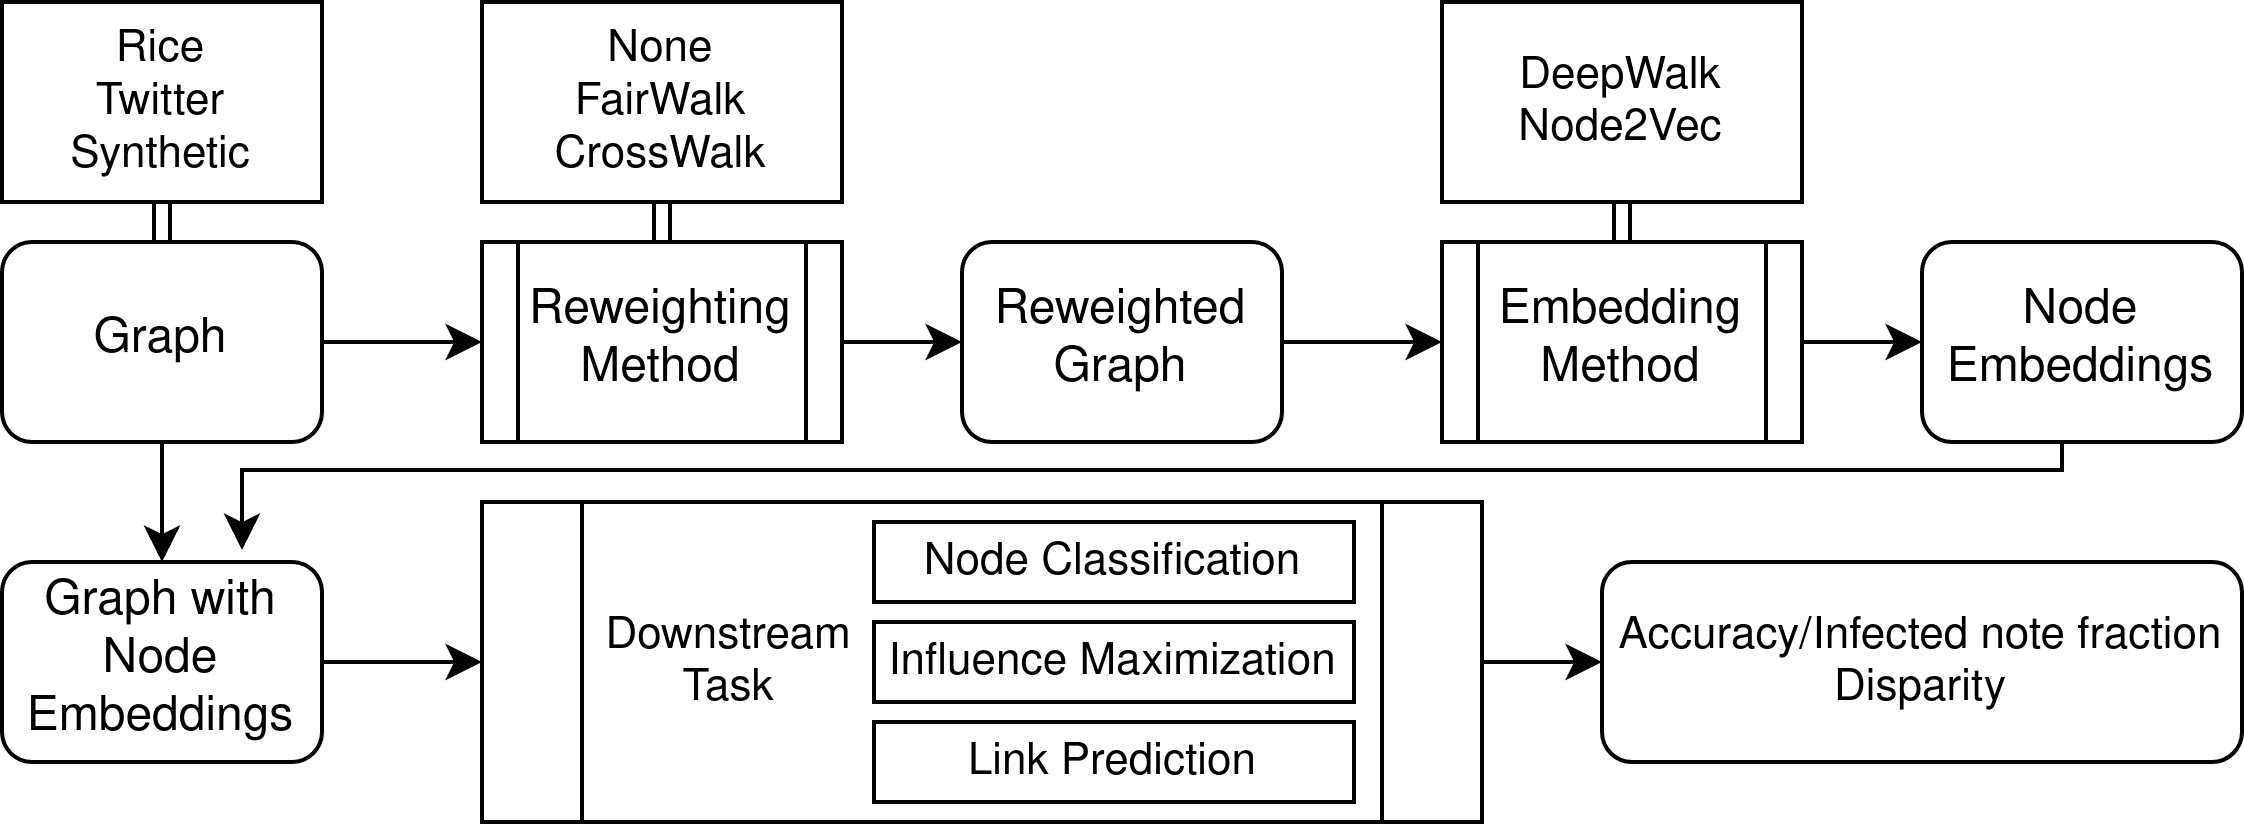
\includegraphics[width=0.85\textwidth]{images/graph_pipeline-better.png}
\caption{\textbf{Schematic overview of the experimental pipeline.}}
\label{fig:pipeline}
\end{figure}


\subsection{Datasets}
\label{subsec:datasets}

% % For each dataset include 1) relevant statistics such as the number of examples and label distributions, 2) details of train / dev / test splits, 3) an explanation of any preprocessing done, and 4) a link to download the data (if available).

Like the original authors, we conduct experiments on two subgraphs of real social networks, and two types of synthetic graphs, which we generate anew for each experimental run to obtain more robust results. 
The real-world datasets are part of our publicly available codebase, as well as methods to generate synthetic ones. More information on datasets can be found in \autoref{subsec:datasets-cont}.


% Note that we generate new synthetic graphs
% To mimic the results of the original paper as accurately as possible, we separate the datasets into train and test splits differently depending on the experiment. The precise values can be found in \autoref{subsec:hyperparameters}.

% \subsubsection*{Rice-Facebook dataset}
% After .... TODO pruning .... The Rice-Facebook dataset \cite{Mislove2010} contains 439 nodes (users), with data for each user regarding the id of their college and their age. The sensitive attribute is defined as the  -id and  with their college-ids with their age class is a subset

% \subsubsection*{Twitter dataset}

% % mention splits are different per experiment, see hyperparameter list

\subsection{Fairness-enhancing edge reweighting strategies}

% Include a description of each model or algorithm used. Be sure to list the type of model, the number of parameters, and other relevant info (e.g. if it's pretrained).

The authors propose CrossWalk as an edge reweighting strategy that can be applied to any graph with positive weights to make the embeddings generated by random walks more fair. This step of reweighting the edge weights is not strictly necessary, as uniform probabilities can also be used to generate random walks. In line with the authors, we also implement FairWalk in order to compare CrossWalk to an alternative fairness-enhancing reweighting strategy. More details about FairWalk and its differences to CrossWalk are presented in \autoref{subsec:reweighting-cont}.


\subsection{Node embeddings}

% 2 sentences on node embedding and 1 sentence on random walk based.
To apply machine learning algorithms on the (reweighted) graphs, one route is to learn low-dimensional node representations first and afterwards perform the downstream task on those representations. \citet{Khajehnejad2022} tested CrossWalk on two random walk-based node embedding methods, namely DeepWalk and Node2Vec. These are explained in more detail in \autoref{subsec:embeddings-cont}


\subsection{Downstream tasks and fairness evaluation}
\citet{Khajehnejad2022} tested CrossWalk on three common applications for learning on graphs, namely influence maximization, link prediction and node classification. These are described in more detail in \autoref{subsec:tasks-cont}. 

The results of each of the three tasks can be described by a global performance metric $0 \leq q \leq 1$, e.g. accuracy, and a collection of performances $Q=\{q_i\}$ evaluated on subsets of the data set defined by sensitive attributes.
To obtain a notion of fairness, for each task the disparity $d=var(Q)$ is computed as the (maximum likelihood) estimate of the variance between performances on the different subsets.
Finding embeddings that minimize the disparity captures the notion of fairness that these embeddings should lead to similar performances for samples of each group.


\subsection{Hyperparameters}
\label{subsec:hyperparameters}
% Describe how the hyperparameter values were set. If there was a hyperparameter search done, be sure to include the range of hyperparameters searched over, the method used to search (e.g. manual search, random search, Bayesian optimization, etc.), and the best hyperparameters found. Include the number of total experiments (e.g. hyperparameter trials). You can also include all results from that search (not just the best-found results).

We recovered most of the original authors' hyperparameters not found in the paper by searching their codebase. Hyperparameters for the experiments on the Twitter dataset were missing (see \autoref{subsec:difficult}). All of the hyperparameters we used are specified in \autoref{tab:hyperparameters} and \autoref{tab:crosswalk-hyperparameters}, and in the configuration files in our code-base.

\subsection{Experimental setup and code}
\label{subsec:exp_code}

The code implementing the entire pipeline as described in \autoref{sec:methodology} is structured as Python package.\footnote{\url{https://github.com/jonathan-gerb/crosswalk-reproduction}} Each of the stages is implemeted as a submodule of the package. This simplifies the conduct of ablation studies with e.g. different datasets by future researchers. The main file of the package takes in one or more configuration files describing the experiments, calls the submodules to perform the total experiment pipeline, and writes the results to .csv files. Runs can be repeated and averaged over multiple trials. Default hyperparameters are defined in a general defaults.py file and can be overwritten by configuration files. We provide the configuration files for all experiments referenced in this paper.

% Include a description of how the experiments were set up that's clear enough a reader could replicate the setup. Include a description of the specific measure used to evaluate the experiments (e.g. accuracy, precision@K, BLEU score, etc.). Provide a link to your code.

\subsection{Computational requirements}
% Include a description of the hardware used, such as the GPU or CPU the experiments were run on. For each model, include a measure of the average runtime (e.g. average time to predict labels for a given validation set with a particular batch size). For each experiment, include the total computational requirements (e.g. the total GPU hours spent). (Note: you'll likely have to record this as you run your experiments, so it's better to think about it ahead of time). Generally, consider the perspective of a reader who wants to use the approach described in the paper --- list what they would find useful. 

All experiments were ran on the CPU of a desktop with an i5-9600K @ 3.70GHz CPU and 32GB of RAM (13GB utilized). The mean runtime per experiment trial was $\sim$30 seconds for the Rice-Facebook and $\sim$13 seconds for 2- and 3-group synthetic datasets. The total runtime for reproducing all the experiments with 50 trials was $\sim$11 hours.

% For the reproduction results Gensim \cite{rehurek_lrec}, which implements word2vec efficiently on CPU was used for the production of node embeddings and thus the GPU was not utilized for the results in this paper.
% jonathan writes

\section{Results}
\label{sec:results}

% Start with a high-level overview of your results. Do your results support the main claims of the original paper? Keep this section as factual and precise as possible, reserve your judgement and discussion points for the next "Discussion" section. 

To confirm the main claims of \citet{Khajehnejad2022} presented in \autoref{sec:claims}, we turn to the two synthetic graphs and the Rice-Facebook dataset. Overall, we find that the results reported by the original authors are statistically plausible. However, we also find that many of them are plagued by high variation of the disparity metric. In an extension of the original paper, we take notice of the importance of hyperparameter tuning when applying CrossWalk.

\subsection{Results reproducing original paper}

% For each experiment, say 1) which claim in Section~\ref{sec:claims} it supports, and 2) if it successfully reproduced the associated experiment in the original paper. For example, an experiment training and evaluating a model on a dataset may support a claim that that model outperforms some baseline. Logically group related results into sections. 

The results of the full range of experiments performed as part of the reproduction study are reported next to their counterparts from the original paper in \autoref{tab:results-reproduction}. Additionally, we provide visualizations of our results in \autoref{fig:visualization-results} in the appendix. We successfully reproduced almost all of the experiments presented in the original paper. However, we were unable to reach comparable results for the Twitter dataset for reasons noted in \autoref{subsec:difficult}. We relegate these results to \autoref{sec:twitter-results}.

\begin{table}[!tb]
    \centering
    \resizebox{\textwidth}{!}{\begin{tabular}{lllrrrr}
        \toprule
        \textbf{Task} & \textbf{Dataset} & \textbf{Embeddings} & \multicolumn{2}{c}{\textbf{Influence/accuracy}} & \multicolumn{2}{c}{\textbf{Disparity}} \\
        & & & \textbf{Original} & \textbf{Reproduced} & \textbf{Original} & \textbf{Reproduced} \\
        \midrule
        IM & 2-group synthetic & DW    & $\sim$12.00 & 10.93 (1.08) & $\sim$48.00 & 44.61 (14.44) \\
           &                   & FW+DW & $\sim$12.00 & 11.07 (0.99) & $\sim$37.00 & 43.35 (14.24) \\
           &                   & CW+DW & $\sim$11.00 & 10.27 (0.73) & $\sim$1.00 & 3.04 (3.70) \\
        \cmidrule{2-7}
           & 3-group synthetic & DW    & $\sim$10.00 & 10.56 (0.74) & $\sim$46.00 & 37.59 (12.91) \\
           &                   & FW+DW & $\sim$10.50 & 10.40 (0.77) & $\sim$30.00 & 26.32 (10.20) \\
           &                   & CW+DW & $\sim$10.00 & 10.16 (0.81) & $\sim$16.00 & 9.87  (8.24) \\
        \cmidrule{2-7}
           & Rice-Facebook & DW    & 18.13 & 17.90 (2.20) & 46.70 & 51.07 (24.64) \\
           &               & FW+DW & 18.20 & 18.47 (1.91) & 20.25 & 25.55 (12.73) \\
           &               & CW+DW & 17.89 & 18.62 (2.22) & 1.36  & \textbf{22.55 (18.74)} \\
        \cmidrule{3-7}
           &               & N2V    & 18.28 & 18.48 (1.79) & 51.88 & 65.54 (26.46) \\
           &               & FW+N2V & 18.03 & 18.49 (2.01) & 18.29 & 25.93 (18.21) \\
           &               & CW+N2V & 18.01 & 17.67 (2.19) & 16.87 & 11.33 (10.45) \\
        \midrule
        NC & Rice-Facebook & DW    & 84.95 & 83.69 (3.05) & 171.01 & 168.82 (87.15) \\
           &               & FW+DW & 81.94 & 83.12 (2.38) & 71.37  & 72.03 (44.72) \\
           &               & CW+DW & 80.72 & 83.35 (2.72) & 58.69  & 71.60 (54.71) \\
        \midrule
        LP & Rice-Facebook & DW    & 76.79 & \textbf{85.92 (0.53)} & 38.91 & \textbf{25.97 (9.83)} \\
           &               & FW+DW & 74.66 & \textbf{84.31 (0.52)} & 13.77 & 11.17 (3.51) \\
           &               & CW+DW & 73.26 & \textbf{83.63 (0.48)} & 3.75  & \textbf{11.07 (4.06)} \\
        \bottomrule
    \end{tabular}}
    \caption{\textbf{Reproduction results.} Comparison of original results and their reproduced counterparts. The table contains results for influence maximization (IM), node classification (NC), and link prediction (LP). We use DeepWalk (DW) and Node2Vec (N2V) embeddings either without reweighting, with FairWalk (FW), or with CrossWalk (CW). Original results over 5 runs were gathered from the original code-base. Unavailable values (preceded by '$\sim$') were estimated from plots in the paper. Reproduced results over 50 runs are presented with standard deviations in parentheses. For original results deviating by more than one standard deviation, the reproduced results are in \textbf{bold}.}
    \label{tab:results-reproduction}
\end{table}

% {Claim 1: Fairness-enhancing property} The authors claim that the application of CrossWalk in all the experiments referenced above leads to enhanced fairness as measured by disparity, compared to both FairWalk and no reweighting-strategy as baselines.

% {Claim 2: Performance-conserving property} The authors claim that the application of CrossWalk in all the experiments referenced above only leads to very small decreases in performance. We interpret this as the performance of every experiment is reduced by at most 10\% when applying crosswalk, compared to both FairWalk and no reweighting-strategy as baselines.

Looking at \autoref{tab:results-reproduction}, one can see that the reproduced values generally validate those reported in the original paper. For the influence maximization and node classification tasks, all but one of the original results fall within one standard deviation of our reproduced results carried out over 50 independent runs. For the link prediction task, the differences are much starker: in terms of accuracy, we find significant improvement over the original results; in terms of disparity, we find significantly lower values when not applying any reweighting strategy and higher values when using CrossWalk.

Focusing on the performance metrics, we see no statistically significant differences between the results obtained with and without CrossWalk. This observation is in line with the one made by the original authors. \textbf{In particular, these results provide evidence in support of the performance-conserving property (Claim 2) of CrossWalk.} However, we see one exception in the case of link prediction performed on the Rice-Facebook dataset, where a significant drop in total accuracy can be observed when a fairness-enhancing reweighting strategy is applied.

Disparity is the original authors' fairness metric of choice. In general, the results presented in \autoref{tab:results-reproduction} show that mean disparity lowers significantly when a reweighting strategy, either FairWalk or CrossWalk, is employed. When performing influence maximization on the two synthetic datasets, we also see a significant improvement of CrossWalk over FairWalk. However, performing downstream tasks on the Rice-Facebook dataset results in statistically insignificant differences between the two, with the only large improvement margin appearing for Node2Vec embeddings. \textbf{Thus, we find inconclusive evidence of the fairness-enhancing property (Claim 1).} In particular, because of large variability of disparity results, the claim of the original authors that CrossWalk consistently provides significant improvement over FairWalk is not supported by the reproduced results.

\subsection{Results beyond original paper}
\label{subsec:sweep}

% Often papers don't include enough information to fully specify their experiments, so some additional experimentation may be necessary. For example, it might be the case that batch size was not specified, and so different batch sizes need to be evaluated to reproduce the original results. Include the results of any additional experiments here. Note: this won't be necessary for all reproductions.

 % TODO: Shorten or split  paragraph belwo by parameter 
While we find insufficient evidence of CrossWalk outperforming FairWalk when dealing with the Rice-Facebook dataset, we argue that CrossWalk may simply require additional hyperparameter tuning. We perform a manual search for the influence maximization task on the dataset for both $\alpha$ and $p$ (see \autoref{sec:crosswalk}).
% \begin{compactenum}
%     \item $\alpha$, which controls the degree in which inter-group and intra-group connections are strengthened and weakened, respectively.
%     \item $p$, which controls the degree of biasness of weights towards visiting nodes at group boundaries.
% \end{compactenum}
%We study the effect of tuning these parameters by performing a sweep over different values and comparing the performance on the influence maximization task for the Rice-Facebook dataset. 
From the results in \autoref{fig:paramsweep}, we observe that increasing $\alpha$ can greatly decrease disparity at an insignificant cost in performance. An opposite pattern emerges when we lower $p$ from the suggested value of 4 to 1, with a lower $p$ resulting in an increase in disparity. Clearly, it is necessary to tune both hyperparameters per experiment in order to find the desired balance between performance and disparity. Importantly, the results are in favor of the \textbf{fairness-enhancing property (Claim 1)} as with a correct choice of hyperparameters, we achieve a significant improvement over FairWalk.
% We additionally perform similar sweeps for the $walk$ $length$ and $walks$ $per$ $node$ hyperparameters from which we can conclude that an increase in walk length can increase accuracy slightly at the cost of disparity. The $walks$ $per$ $node$ experiment yielded inconclusive results, see Appendix \autoref{fig:paramsweep2} for the full results.

\begin{figure}[!htbp]
    \centering
   \subfloat[Hyperparameter $\alpha$]{
   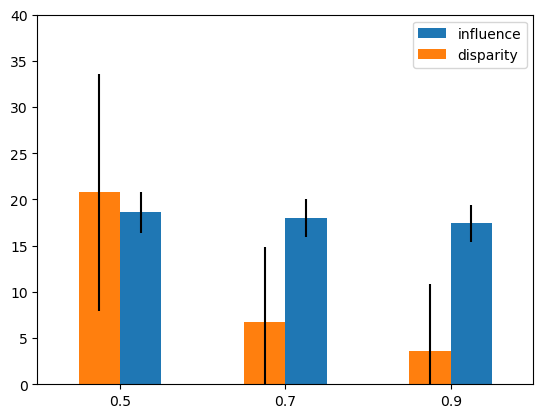
\includegraphics[width=0.40\textwidth]{images/paramsweeps/alpha_sweep.png}}
   \subfloat[Hyperparameter $p$]{
   \includegraphics[width=0.40\textwidth]{images/paramsweeps/p_sweep.png}}
\caption{\textbf{Impact of hyperparameters $\alpha$ and $p$ (beyond the original paper).} Influence and disparity for influence maximization on the Rice-Facebook dataset for different $p$ and $\alpha$ values on the influence maximization task. One can observe that the trade off between accuracy and disparity can be tuned using these hyperparameters.}
\label{fig:paramsweep}
\end{figure}

% \subsubsection*{Handling of edge cases in CrossWalk algorithm}

% \subsubsection*{Robustness of Crosswalk Against Training Setup}


%Even though we used the same hyperparameters as them we were not able to reproduce the exact same results as them. Investigating their code-base shows that seeds were not systematically passed and that the standard deviations although not reported were quite large. However, we do find that their results are statistically plausible. \textbf{Claim 1: Fairness-enhancing property} and \textbf{Claim 2: Performance-conserving property} hold for all experiments. The reproduction results are obtained using their parameters. In our additional results we show that for our implementation other hyperparameters would lead to lower disparities and the importance in general of tuning for crosswalk.


\section{Discussion}
\label{sec:discussion}

% Give your judgement on if your experimental results support the claims of the paper. Discuss the strengths and weaknesses of your approach - perhaps you didn't have time to run all the experiments, or perhaps you did additional experiments that further strengthened the claims in the paper.

Putting our findings presented in \autoref{sec:results} into context, we believe that the main claims of the authors presented in \autoref{sec:claims} are supported and strengthened by our reproduction study. We find strong evidence in support of the \textbf{performance-conversion property (Claim 2)} of CrossWalk. And while we find only limited evidence in support of CrossWalk providing significant improvement in disparity over FairWalk when performing tasks on the Rice-Facebook dataset, we confirm that with additional hyperparameter tuning, the \textbf{fairness-enhancing property (Claim 1)} holds even in this case.

Moreover, we believe in our results providing strong support for CrossWalk due to our choices to (1) re-implement CrossWalk from scratch using trusted packages, such as PyTorch, DGL, and scikit-learn, thus minimizing the chances of common mistakes, (2) perform all experiments over 50 runs (rather than the original authors' 5 runs) and take into consideration the variability of the disparity measure, and (3) extend CrossWalk in order to provide better guarantees and graceful handling of more edge cases while having no big impact on the results, as can be seen in \autoref{fig:ours-vs-theirs} in the appendix.

% The results from  \autoref{sec:results} confirm and strengthen the main claims of the authors, as discussed in \autoref{sec:claims}, for three reasons:\\
% \textbf{1. Re-implementation.} We reproduce the same trends as the original authors with an independent implementation based on trusted packages like PyTorch, DGL, gensim and sklearn, thus minimizing the chances of common mistakes.\\
% \textbf{2. Robustness check.} We ran all experiments for 50 trials, compared to 5 trials in the original paper and report standard deviations. Given that the standard deviations for disparity are large, this is necessary to verify the claims. \\
% \textbf{3. Theoretical extension.} Extending CrossWalk as discussed in \autoref{sec:crosswalk} provides better guarantees and graceful handling of more edge cases while having no big impact on the results, as can be seen in \autoref{fig:ours-vs-theirs} in the appendix.

% \begin{enumerate}
%     \item \textbf{Re-implementation.} With an independent code-base we manage to reproduce the same trends as them. Our code-base outsources all parts, that are not CrossWalk and FairWalk, to well established packages like PyTorch, DGL, gensim and sklearn. Therefor the results are very transparent and it will be easier for other researchers to use our implementation.
%     \item \textbf{Robustness check.} All experiments were ran for 50 trials, compared to 5 trials in the original paper. Given that the standard deviations for disparity are large this is very important to verify the claims.
%     \item \textbf{Theoretical extension.} Our extended version of CrossWalk as discussed in \autoref{sec:crosswalk} gives the same results as their version as can be seen in \autoref{fig:ours-vs-theirs} and it also handles more edge cases.
% \end{enumerate}


\subsection{Further work} 
% As discussed in \autoref{subsec:sweep}, the hyperparameters have a large influence on the results. Because the data was different from the original paper and hyperparameters were missing for the Twitter dataset we were not able to reproduce the results for that dataset. 
% However, with our highly modular package other researchers can easily try different datasets and experiments.
We believe that the largest of our contributions is the highly-modular implementation. We hope that researchers will employ it for future research to easily evaluate the impact of CrossWalk on different datasets, tasks, and fairness metrics. In the same sense, variations of CrossWalk, obtained, for example, changing the definition of colorfulness, can be implemented and extensively tested by changing just a few lines.


\subsection{What was easy}

% Give your judgement of what was easy to reproduce. Perhaps the author's code is clearly written and easy to run, so it was easy to verify the majority of original claims. Or, the explanation in the paper was really easy to follow and put into code. 

% Be careful not to give sweeping generalizations. Something that is easy for you might be difficult to others. Put what was easy in context and explain why it was easy (e.g. code had extensive API documentation and a lot of examples that matched experiments in papers).

% 1. their code-base 
% 2. theory is easy

The original paper is accompanied by a code-base to run all experiments. The implementation, and especially some of its unit tests, were of much help in understanding the methods in more detail. The pseudocode in the original paper was helpful, too.
In contrast to FairWalk, the authors proposed CrossWalk as a reweighting method. Thereby, they decoupled it from the generation of random walks. This subtle but important change of perspective allowed for a modular implementation with higher flexibility and testability.

\subsection{What was difficult}
\label{subsec:difficult}

% List part of the reproduction study that took more time than you anticipated or you felt were difficult. 

% Be careful to put your discussion in context. For example, don't say "the maths was difficult to follow", say "the math requires advanced knowledge of calculus to follow".

% A full overview of all difficulties faced while re-implementing the results and our respective contributions is given in \autoref{tab:issues}. 

\subsubsection*{Difficulties regarding the paper}
As detailed in \autoref{sec:crosswalk}, the CrossWalk formula, pseudo-code, and actual implementation were not aligned, which made reproduction difficult. This was amplified by some notational inconsistencies. Lastly, the presentation of the results in the paper lacked exact numbers and standard deviations. 

% Therefor it was impossible for us to directly confirm if their results were statistically plausible given our results. 
\subsubsection*{Difficulties regarding the data}
The Rice-Facebook dataset in the code-base did not include all attributes needed to perform the node classification task. To perform the task, we had to track were the data came from and supply it ourselves. 
We could not reproduce the experiments on the Twitter dataset, because the version that was available differed from the description in the paper (see \autoref{subsec:datasets-cont} in the appendix) and because the original hyperparameters were missing.
% Moreover, the Twitter dataset was not available in the form described in the paper, as described in \autoref{subsec:datasets-cont}. Additionally, there was no bash file included to run the experiment, so we could not access the original hyperparameters as described in \autoref{subsec:hyperparameters}. 
Instead, we ran the experiments on the dataset that was provided in the code-base with the hyperparameters for the Rice-Facebook dataset. The results, presented in \autoref{sec:twitter-results}, did not live up to expectation. However, this may be alleviated with hyperparameter tuning.

\subsubsection*{Difficulties regarding the code}
The provided code-base came without a license, hindering accessibility. 
% We understand that the code-base was developed 
Further issues include: lack of documentation, inconsistent variable naming, hard-coded hyperparameters, missing environment specifications and no seeding methods being used for reproducibility. Lastly, to re-run one experiment end-to-end with the original code-base, we had to guess the necessary yet undocumented process of identifying files containing partial results, moving them to different folders twice and copying the printed results into a notebook.

\subsection{Communication with original authors}

% Document the extent of (or lack of) communication with the original authors. To make sure the reproducibility report is a fair assessment of the original research we recommend getting in touch with the original authors. You can ask authors specific questions, or if you don't have any questions you can send them the full report to get their feedback before it gets published. 

Due to the absence of an open-source license in the original code repository, we initially reached out to the original paper's authors to ensure we could use their code. Furthermore, we wished to gain insight into some of their design choices. We received a prompt response providing assurance about the code use and the needed explanations.





% NOTES FROM CONVERSATION

% Kieron: January 26, 14:52
% 1. For CrossWalk experiments it seems that we use randomly initialized priors when we shouldn't.
% - Default (and not overwritten for synth data experiments): _C.SYNTHETIC.INIT_WEIGHTS = True 
% -> This creates random (!!!) weights that follow a gamma distribution in ndata["weights"]. The author's never do this, I implemented the parameter init_random_weights just for testing.
% - Default (and not overwritten for synth data experiments): _C.GRAPH_KEYS.PRIOR_WEIGHTS_KEY = 'weights'
% -> This uses those random weights as prior for crosswalk
% Suggestion Option 1.1: Change type of _C.SYNTHETIC.INIT_WEIGHTS to string with the following options:
% - Default: "uniform" (that is probably what you thought this does)
% - Alternative option would be "gamma" (never used for experiments): 

% Option 1.2:
% - Set defaults to INIT_WEIGHTS=False and PRIOR_WEIGHTS_KEY=None
% - This also leads to a uniform prior, because I have implemented CrossWalk to assume that if no prior weights are specified

% 2. If we do 'skip' than the prior weights are used leading to the random gamma weights that we do not want (see issue 1).
% - Would be solved if we decide for Option 1.1, because then we'd have uniform weights
% - If we decide for Option 1.2 then we need to confirm that deepwalk, node2vec all work without any prior weights (iirc dgl's node2vec does assume a uniform prior if none is provided)

% I'm a bit overwhelmed right now, so I might go off the rails a bit. but I'm considering whether we should make that clear somewhere. Not sure if it's a thing for readme and/or report. 

% I looked at the CrossWalk paper, and they also seem to share that interpretation of cross- and FairWalk being "reweighting" strategies rather than "walking" strategies. This being valid is confirmed by dgl's node2vec implementation having a parameter for passing prior weights.

% I think I'm just confused because FairWalk paper never talks about weights

% i'll leave this for now and focus on refactoring. maybe @Eric Zila has already made that distinction clear in the intro, or maybe it's not even worth mentioning

% also... Do we know whether they also removed the parallel edges? Their implementation is different, so they might have kept them.

% This would lead to higher infection numbers than we'll ever be able to reproduce. I really don't want to investigate right now, but imo this needs to be at least mentioned in our report